\newpage
\section{Binary Watch}
\subsection{PCB}
\subsubsection{First PCB Version}
The First PCB Version was a desaster. The PCBs arrived very fast, but the QFN Package had the wrong size.
ATMEL only produces QFN32 in 7x7mm. Therefore the design of the PCB hat to be changed to the smaller package,
but that gave me the Chance to shrink the Design to a smaller form factor.
The part which keeps the PCB from getting smaller is the Coin Cell Battery (CR2032).
On the PCBs there was the order number printed on the Front side, which would be visble in the final assembly.
\subsubsection{Second PCB Version}

The second PCB Version was designed from scratch. But the Front was the side with the Battery, so hopefully the Order Number would not be printed on the visible side of the PCB. This worked out very well for the second Version of the PCBs.
\subsubsection{PCB1}

since the PCBs finally arrived. it was possible to assemble all the parts.
The first PCB was assembled with some Cables soldered to the Testpins on the Backside of the Board.
And the Battery case was also not assembled.
Here is a Picture of the uncleaned but already soldered PCB
\begin{center}
  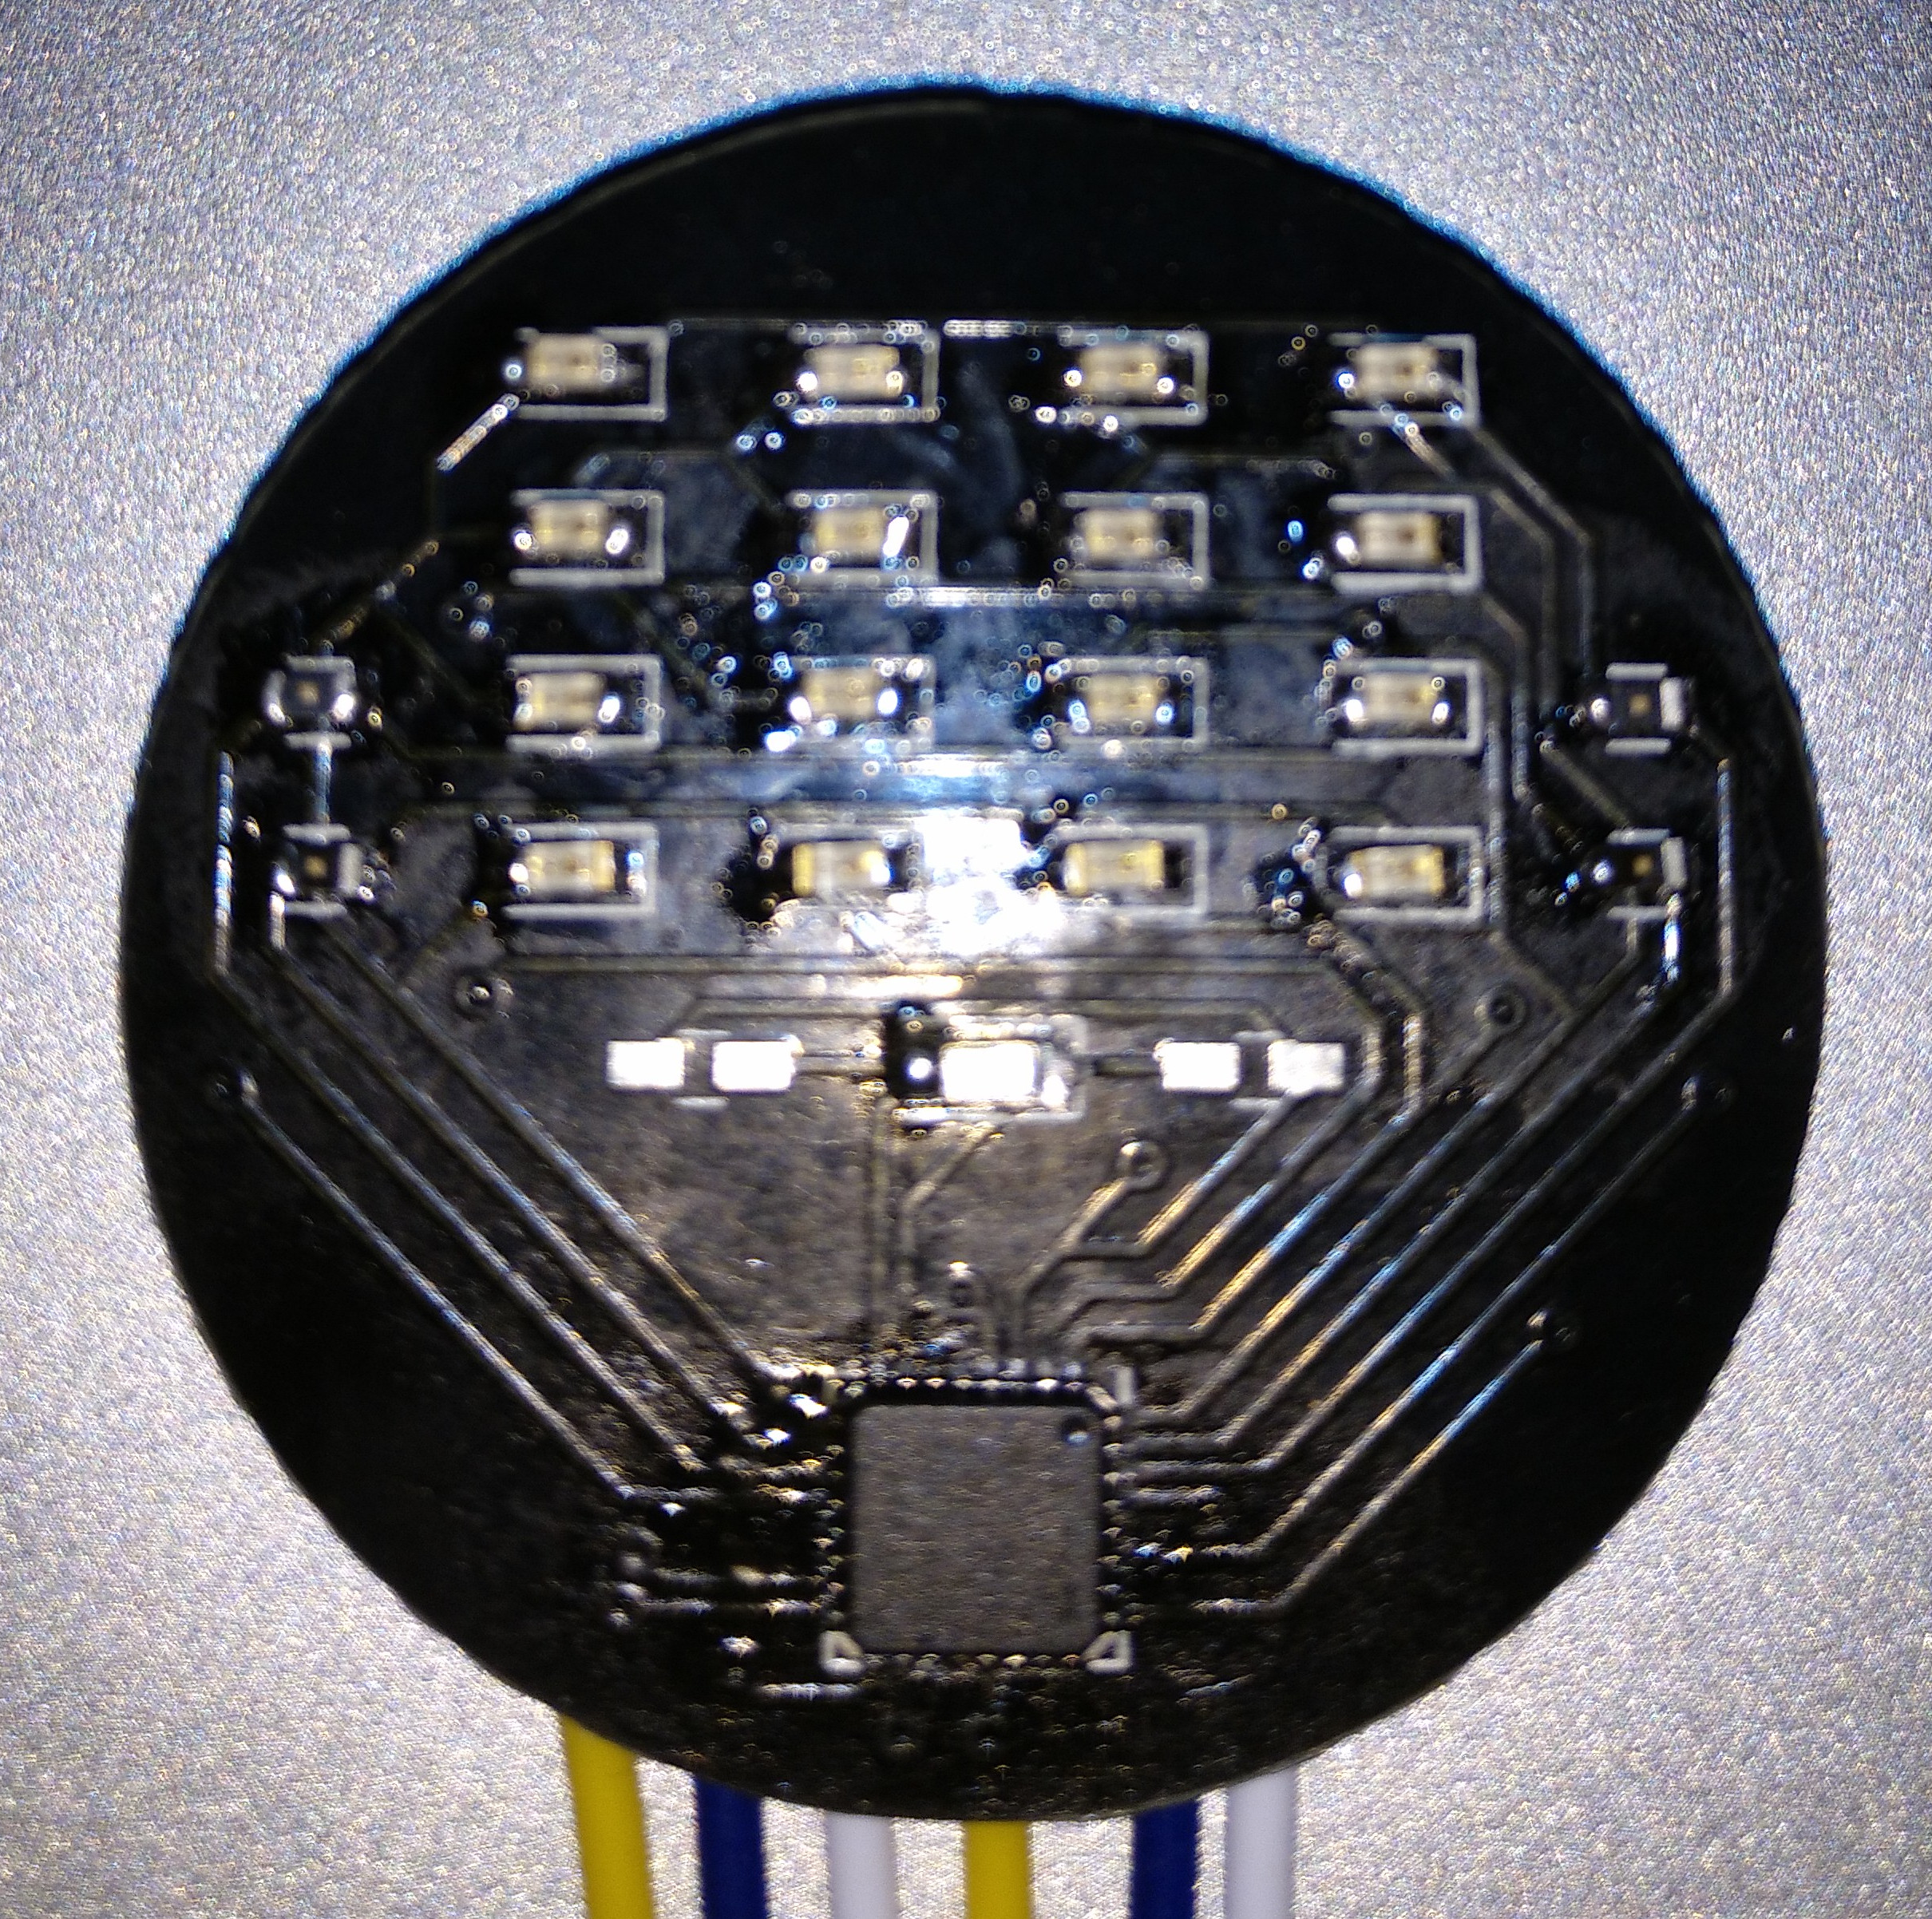
\includegraphics[width=0.5\textwidth]{../Pictures/PCB1_F1.jpg}
\end{center}

\subsubsection{PCB2}
The PCB2 was assembled and cleaned as a First Prototype with the Housing.\
Here aretwo Pictures of the PCB one without the LEDs turned on and one with the LEDs turned on.\
Brightness was set in the Program to 100/255 (see software void showLEDs, constant perc=100) 
\begin{center}
\includegraphics[width=0.45\textwidth]{../Pictures/PCB2_F1_off.jpg} \includegraphics[width=0.45\textwidth]{../Pictures/PCB2_F1_on.jpg}

\end{center}

\subsubsection{PCB3}
The third PCB was ordered at \href{https://aisler.net}{aisler.net}. It only took around one and a half week to arrive(to Germany).\
The PCB was not completely milled out. It was in a carrier PCB with rectangular shape, but it was easy to remove.\
I had to sand the edges a bit, since it was a bit rough on the parts where i removed the connections to the carrier, since i had to sand the PCB anyway to fit in the Housing that was no big problem.\
The overall Quality of the PCBs is very good, but you can not choose the thicknes or color of the PCB.\
\begin{center}
  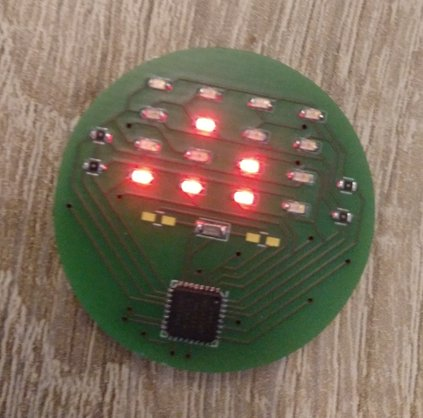
\includegraphics[width=0.5\textwidth]{../Pictures/PCB3.jpg}
\end{center}

\newpage

\subsection{Housing}
The Housing was designed in OpenSCAD.\
a very helpfull reference for the OpenSCAD syntax was\
\url{https://en.wikibooks.org/wiki/OpenSCAD_User_Manual/Transformations}

\subsubsection{Housing 1}
The Housing was printed by the TOOM Printing Service as SLS in PLA.\
Sadly all the surfaces are not really smooth, therefore the Buttons are working very bad.\
I tried to glue in the glass with superglue, but the glue dried out white, this looks really bad :-(\

\subsubsection{Plans for Housing 2}
The next housing should be produced via SLA with transparent Resin, so no glass for Protection is needed, 
since the resin could be used.
\paragraph{Problems while printing with SLA}
It turns out, that there is no completely transparent Resin available. All of them get a yellow color sooner or later.
So it is not really beautiful as a glass.

\subsubsection{Housing 2}
A friend told me that most of the time the resin will not reflect light equally in every spot, therefore i decided to order a PCB without glass and do the mounting of the glass with very tight tolerances and a rim on the top edge.\
this worked out extremely well.\
Another goal was to make the second Housing slim, because the first one was very bulky. With a bit of optimization is was possible to integrate the bottom plate completely in the housing. The overall thicknes was reduced from about 15mm to 9.4mm with the 1mm PCB or 10mm with the new 1.6mm PCB.\
For the PCB to tightly fit in either the Housing has to get some aditional holes or at least the Battery clip has to be modified.\
\begin{center}
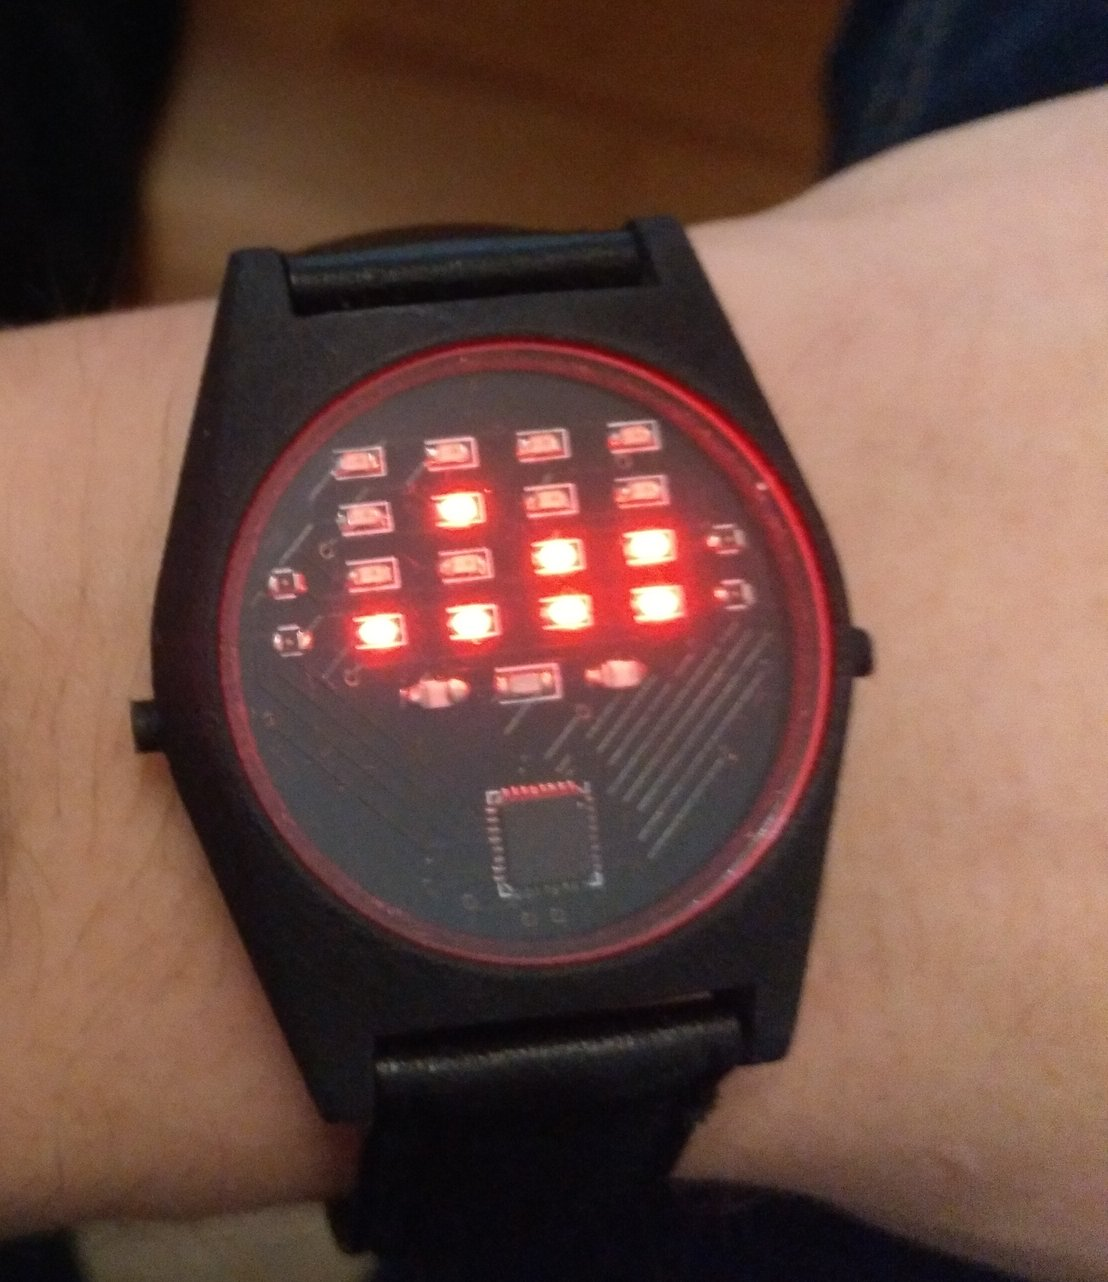
\includegraphics[width=0.45\textwidth]{../Pictures/Housing2.jpg} 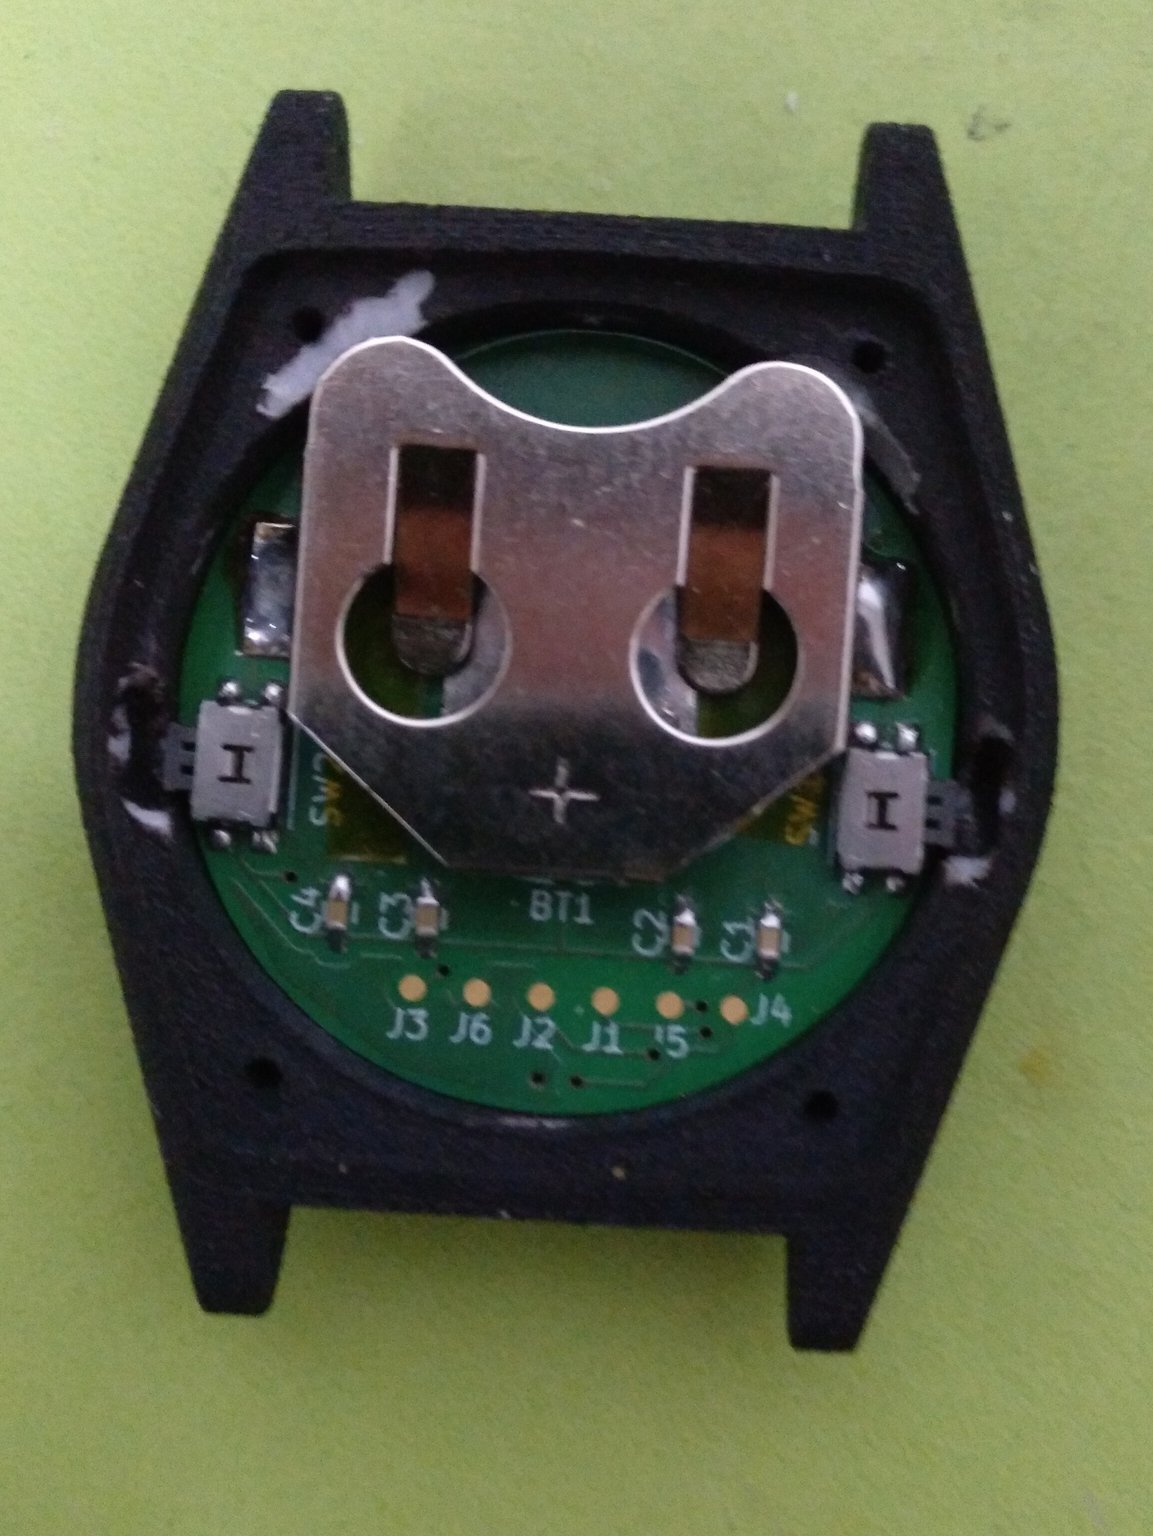
\includegraphics[width=0.45\textwidth]{../Pictures/Housing3b.jpg}
\end{center}

\subsection{Problems}
\subsubsection{Sweat is entering the Housing}
The first watch broke down after nearly 1 year. After opening the Housing the Problem was very obvious. Sweat was entering the Housing and corroded the PCB and the mounted parts.
\begin{center}
  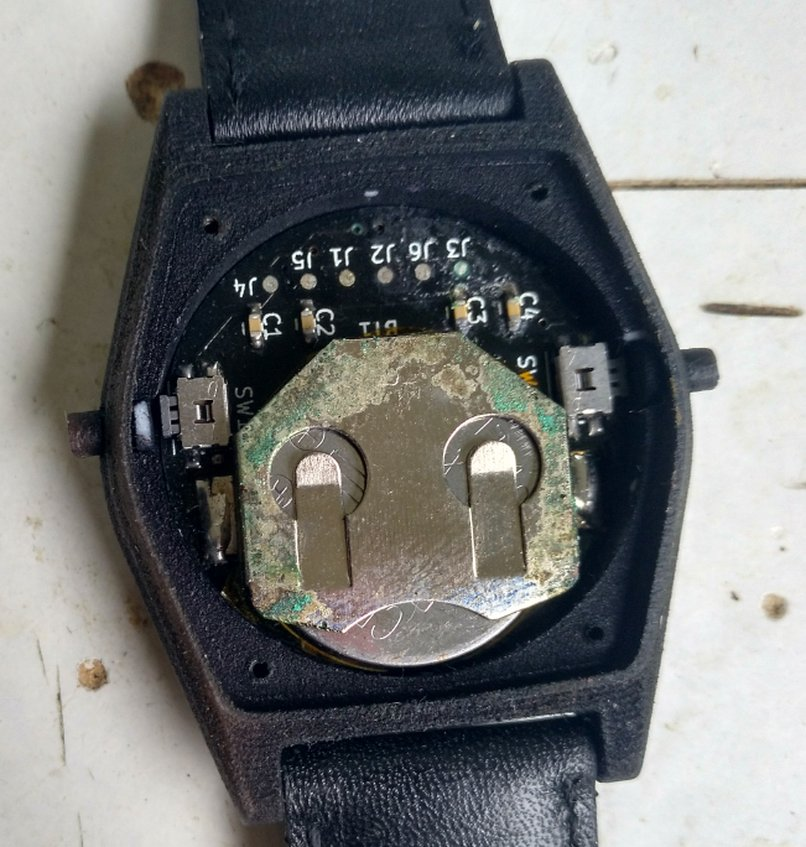
\includegraphics[width=0.5\textwidth]{../Pictures/ProbCorr1.jpg}
\end{center}
\paragraph{Cleaning the PCB and adding something to absorb the moisture}
As a solution i tried to clean the PCB with Isopropanol and glued some rice to the PCB to absorb the moisture, that helped only for about a week and the Watch stopped working again. So that is not the best solution, but is is an extraordinary try ;-)
\begin{center}
  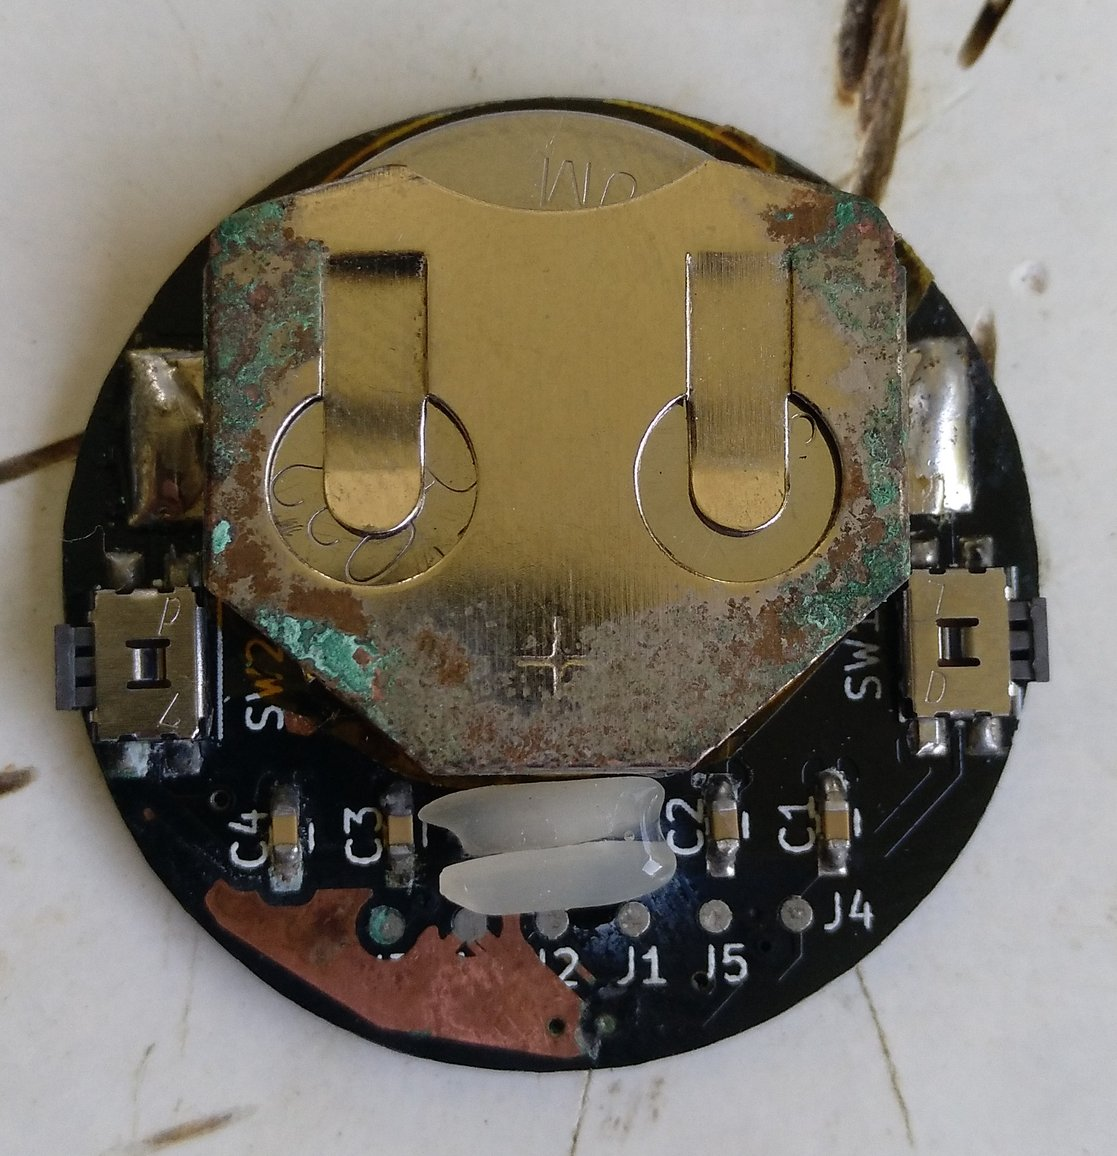
\includegraphics[width=0.5\textwidth]{../Pictures/ProbCorrSol1.jpg}
\end{center}
\paragraph{adding isolation Tape between the lid and the housing}
The second solution was to add Tape, which is originally designed to be used to seal threads, between the housing and the lid.\
That worked out a little bit better, but the Watch also stopped working after a few weeks. 
\paragraph{Analyzing the Watch again}
After analyzing it again the PCB seemd to be ok. The PCB was only a little damaged from the first sweat attack.
The Problem was that the time stopped to run, but another point was that the LEDs wont go off anymore. 
But it was possible to set the time. 
So the conclusion is that the clock which is run by the crystal stopped running.
\paragraph{Adding clear Nailpolish to guard the Crystal}
The next attempted solution was to add clear Nailpolish to the PCB, so the crystal is completely covered. This is an attempt to stop moisture from crawling below the crystal and stopping the clock.

Adding Nailpolish was also not the real solution. The Clock also stopped to work after a few weeks.

\paragraph{commercial products to insulate PCBs}
The next attempt will be to use a commercial Product to insulate the PCB.
For this i will try \href{https://www.reichelt.de/korrosionsschutzlack-plastik-70-super-400-ml-isolierlack-kontakt-32046-p125737.html}{Plastik 70 Super} from Kontakchemie.


\subsection{Manual}
\subsubsection{How to read the Watch}
The time is displayed in BCD Code. For further reference please see the Picture below:
\begin{center}
  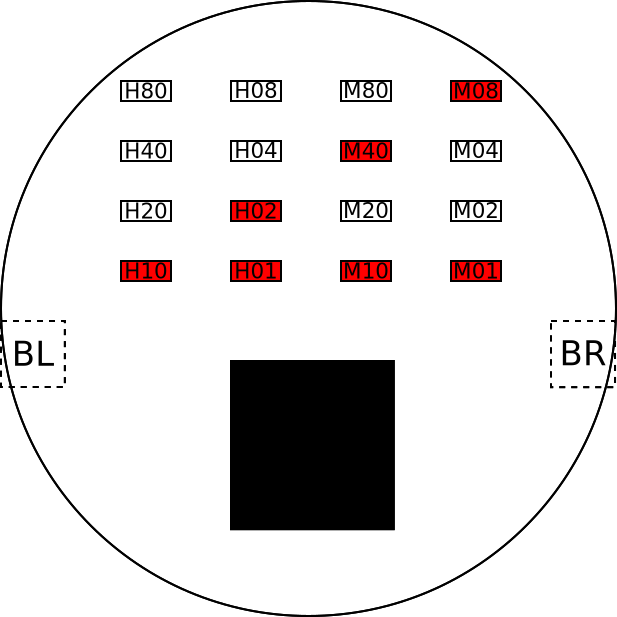
\includegraphics[width=0.5\textwidth]{drawings/BinDia1359.png}
\label{fig:BinWatchFace}
\end{center}
There are Two Buttons on the Watch:
\begin{itemize}
	\item BL: left Button
	\item BR: right Button
\end{itemize}
To read the Watch it is necessary to activate the Display via one of the Buttons

The LEDs are read columnwise. So the right two columns are showing the Minutes. If an LED is litone have to add its Value to the Minutes if not then nothing is added. So for the full hour no led in the right two columns will be lit.

In the Example above the following LEDs are lit: M40, M10, M08 and M01.
The sum of all the values is the current minute value $40+10+8+1=59$

The Hours are displayed exactly like the Minutes. For the hours the 24 Hour Format is used. In the Example above the following LEDs are lit: H10, H01, H02. The current Hour Value is also determined by summing everythin up: $10+1+2=13$.

So the current Time in the example is 13:59. If it is 0:00 the watch will display 24:00 to make sure 0:00 is not confused with a broken watch.
\subsubsection{set the time}
To set the time first of all the display has to be activated, afterwards both buttons have to be released (to make sure that the setup mode is not accessed accidently). Now both buttons have to be pressed. Now the LED H80 lights up, to signalize that now it is in set hour mode. Now Both buttons can be released again.

To switch to the set minute mode the right button has to be pressed. In set minute mode the right button switches back to the normal mode.

With the right button the value which is set currently can be incremented.
The hour will not be incremented wen incrementing the minutes from 59 to 0.

Both setup modes will timeout if no button is pressed for 30 seconds.
While the watch is in setup mode the clock will be stopped, after returning to normal mode the seconds will start from 0 so it is easy to set the time precisely.

